%% 
%% Copyright 2019-2020 Elsevier Ltd
%% 
%% This file is part of the 'CAS Bundle'.
%% --------------------------------------
%% 
%% It may be distributed under the conditions of the LaTeX Project Public
%% License, either version 1.2 of this license or (at your option) any
%% later version.  The latest version of this license is in
%%    http://www.latex-project.org/lppl.txt
%% and version 1.2 or later is part of all distributions of LaTeX
%% version 1999/12/01 or later.
%% 
%% The list of all files belonging to the 'CAS Bundle' is
%% given in the file `manifest.txt'.
%% 
%% Template article for cas-dc documentclass for 
%% double column output.

%\documentclass[a4paper,fleqn,longmktitle]{cas-dc}
\documentclass[a4paper,fleqn]{cas-dc}

%\usepackage[numbers]{natbib}
%\usepackage[authoryear]{natbib}
\usepackage[authoryear,longnamesfirst]{natbib}

%%%Author definitions
\def\tsc#1{\csdef{#1}{\textsc{\lowercase{#1}}\xspace}}
\tsc{WGM}
\tsc{QE}
\tsc{EP}
\tsc{PMS}
\tsc{BEC}
\tsc{DE}
%%%

% Uncomment and use as if needed
%\newtheorem{theorem}{Theorem}
%\newtheorem{lemma}[theorem]{Lemma}
%\newdefinition{rmk}{Remark}
%\newproof{pf}{Proof}
%\newproof{pot}{Proof of Theorem \ref{thm}}

\begin{document}
\let\WriteBookmarks\relax
\def\floatpagepagefraction{1}
\def\textpagefraction{.001}

% Short title
\shorttitle{Leveraging social media news}

% Short author
\shortauthors{CV Radhakrishnan et~al.}

% Main title of the paper
\title [mode = title]{A Systematic Comparison of Reservoir Computing Frameworks}                      
% Title footnote mark
% eg: \tnotemark[1]
%\tnotemark[1,2]

% Title footnote 1.
% eg: \tnotetext[1]{Title footnote text}
% \tnotetext[<tnote number>]{<tnote text>} 
\tnotetext[1]{This document is the result of a research
   project funded by Teuscher Lab.}


% First author
%
% Options: Use if required
% eg: \author[1,3]{Author Name}[type=editor,
%       style=chinese,
%       auid=000,
%       bioid=1,
%       prefix=Sir,
%       orcid=0000-0000-0000-0000,
%       facebook=<facebook id>,
%       twitter=<twitter id>,
%       linkedin=<linkedin id>,
%       gplus=<gplus id>]
\author[1,3]{Nihar Koppolu}[type=editor,
                        auid=000,bioid=1,
                        orcid=0000-0001-7511-2910]

% Corresponding author indication
\cormark[1]

% Footnote of the first author
\fnmark[1]

% Email id of the first author
\ead{cvr_1@tug.org.in}

% URL of the first author
\ead[url]{www.cvr.cc, cvr@sayahna.org}

%  Credit authorship
\credit{Conceptualization of this study, Methodology, Software}

% Address/affiliation
\affiliation[1]{organization={Elsevier B.V.},
    addressline={Radarweg 29}, 
    city={Amsterdam},
    % citysep={}, % Uncomment if no comma needed between city and postcode
    postcode={1043 NX}, 
    % state={},
    country={The Netherlands}}

% Second author
\author[2,4]{Han Theh Thanh}[style=chinese]

% Third author
\author[2,3]{CV Rajagopal}[%
   role=Co-ordinator,
   suffix=Jr,
   ]
\fnmark[2]
\ead{cvr3@sayahna.org}
\ead[URL]{www.sayahna.org}

\credit{Data curation, Writing - Original draft preparation}

% Address/affiliation
\affiliation[2]{organization={Sayahna Foundation},
    % addressline={}, 
    city={Jagathy},
    % citysep={}, % Uncomment if no comma needed between city and postcode
    postcode={695014}, 
    state={Trivandrum},
    country={India}}

% Fourth author
\author%
[1,3]
{Rishi T.}
\cormark[2]
\fnmark[1,3]
\ead{rishi@stmdocs.in}
\ead[URL]{www.stmdocs.in}

\affiliation[3]{organization={STM Document Engineering Pvt Ltd.},
    addressline={Mepukada}, 
    city={Malayinkil},
    % citysep={}, % Uncomment if no comma needed between city and postcode
    postcode={695571}, 
    state={Trivandrum},
    country={India}}



% Here goes the abstract
\begin{abstract}
In this paper, we conducted a comprehensive evaluation of five reservoir computing software simulation frameworks. Reservoir computing (RC), a specialized machine learning algorithm, employs fixed, nonlinear systems to map signals into higher dimensions. Its primary advantage lies in training only the readout layer, expediting learning and accommodating various physical implementations. The growing interest in RC has led to the development of many RC simulation frameworks. There is no other systematic comparison of the different RC frameworks, making our evaluation particularly relevant. The frameworks reservoirpy, RcTorch, pyRCN, pytorch-esn, and ReservoirComputing.jl - were assessed based on their features, applications, documentation quality, and performance across three benchmark tasks. Reservoirpy has the most comprehensive set of features that support the design of highly customizable features. The framework with the best performance in terms of overall training time and accuracy was pytorch-esn which is significantly faster than any other framework. This will help researchers simulating RC to decide which framework suits their purposes the best. 


In this paper, we present a thorough examination of five reservoir computing  software simulation frameworks, namely reservoirpy, RcTorch, pyRCN, pytorch-esn, and ReservoirComputing.jl. Reservoir computing (RC), as a specialized machine learning algorithm, leverages fixed, nonlinear systems to map signals into higher dimensions. Its unique strength lies in training only the readout layer, thereby expediting the learning process and accommodating diverse physical implementations. The increasing interest in RC has led to the proliferation of various RC simulation frameworks. However, there exists no systematic comparison of these frameworks, rendering our evaluation particularly pertinent. Our assessment focuses on crucial aspects such as features, applications, documentation quality, and performance across three benchmark tasks. Reservoirpy stands out for its comprehensive set of features, offering unparalleled support for designing highly customizable simulations. Pytorch-esn has the best performance in terms of reducing the training time of simulated RC networks while maintaining high accuracy. This analysis is a valuable resource for researchers simulating RC, aiding in informed framework selection.
\end{abstract}





% Keywords
% Each keyword is seperated by \sep
\begin{keywords}
Reservoir Computer \sep MNIST \sep Mackey-Glass
\end{keywords}

\maketitle


\section{Motivation}
There is an increasing interest in using AI to solve varied problems in a massive array fields such as healthcare, finance, meteorology, etc. Reservoir computing (RC) is a paradigm that allows the construction of unconventional yet simple AI systems from a wide variety of physical substrates. For this reason, there has been an explosion in interest in RC from a broad spectrum of researchers. This interest has led to the development of a number of RC simulation frameworks with different features. It is important for researchers - those who are both have deep knowledge or minimal knowledge pertaining to machine learning -  to be able to decide which RC framework is best suited to their needs. Having a greater understanding of the frameworks that are already available will help researchers more effectively choose specific frameworks and tools that best suite the completion of their tasks. We have assessed the different frameworks and determined their specific applications and differences in performance. We have also created a comprehensive set of tutorials that provide insight on how to use these frameworks. 

ADD MORE ABOUT WHY YOU CHOSE THE SPECIFIC FRAMEWORKS YOU CHOSE AND WHY YOU DID NOT INCLUDE FRAMEWORKS LIKE OGER AND AURESERVOIR

\section{Introduction}
Reservoir computing (RC) is a novel machine learning algorithm that draws inspiration from neural networks and the structural complexity of the brain. Much like an artificial neural network, reservoir computers (RC) utilize an initial input and final output/readout layer. However, RCs are distinguished by only having 3 layers with the central layer being the reservoir which is a recurrent network that allows processing of temporal information. The reservoir layer - inspired by the brain's intricate connectivity - leverages a densely connected network that allows for rich nonlinear transformation of linear signals onto a higher dimensional space \citep{cucchi_hands-reservoir_2022}. RCs have specific advantages in terms of training time and the prospect of physical implementation when compared to traditional neural networks such as feed forward neural networks (FNN) and recurrent neural networks (RNN). The generic structure of each of these machine learning algorithms is depicted below.

\begin{figure}[h!]
    \centering
    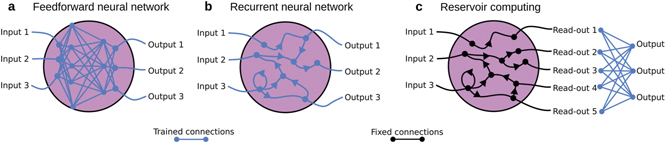
\includegraphics{figs/iop_tutorial_image.jpeg}
    \caption{\citep{cucchi_hands-reservoir_2022}}
    
    \label{fig:enter-label}
\end{figure}

The structure of RCs and RNNs are better suited for handling sequential data in comparison the FNNs. RNNs have recurrent connections that allow them to maintain a hidden state that captures information from previous inputs, allowing RNNs to remember temporal dependencies in a data set \citep{medsker_recurrent_2001}.  The reservoir layer in RCs also have recurrent connections that have the same capability of storing states based on previous input data. In a recent study by \cite{shahi2022prediction}, it was shown that RCs and RNNs are both able to accurately complete timeseries prediction tasks; however RCs required significantly less computation time. What distinguishes a RC from an RNN is that none of the connections including the recurrent connections within the reservoir layer are trained \citep{jaeger2001short}. In a RC architecture, only the connections between the reservoir and the readout layer are trained; training of these connections can be done through the use of a simple linear regression algorithm. FNNs use backpropagation algorithms that require multiple layers of weights to be trained, and the recurrent connections in RNNs are trained through the use of the back propagation through time algorithm which is considered even more computationally expensive. The advantage that RNNs have with a greater number of trainable connections is that they are more adaptable. On the other hand, RCs leverage the inherent dynamics of the reservoir for computation, and their fixed weights contribute to their simplicity and ease of training.

The simple structure of RCs lends itself to physical implementations. The reservoir which does not require adaptive updating can be implemented with unconventional hardware the leverages physical systems, substrates, and devices that are capable of representing dynamical, high-dimensional states for the purposes of computation \cite{cucchi_hands-reservoir_2022}. The variety of physical systems that can be used to implement RCs has led to a broad interest in reservoir computing amongst researchers in diverse fields. The general requirements for both physical and simulated reservoirs to solve computational tasks are the following \citep{tanaka_recent_2019}:
\begin{itemize}
    \item high dimensionality: the ability to map inputs into a higher dimensional space to separate previously inseparable inputs
    \item non-linearity: transforms input data non-linearly which helps with the extraction of non-linear dependencies in the inputs
    \item fading memory: the state of a reservoir must be dependent on recent past inputs with distant inputs being less significant
    \item separation property: the different responses of a reservoir must be separated into distinct signals that can be mapped to a readout layer
\end{itemize}
An example of a novel implementation of a physical reservoir is a fluidic RC in which input signals related to an XOR task are transformed and transmitted using an electric motor that generates ripples in a pool of water that acts as a reservoir layer, and from recordings of these ripples a software based readout is trained. More on this example alongside other examples of physical RC implementations are listed in a survey paper by \cite{tanaka_recent_2019}.


Aside from the diverse set of architectures associated with physical implementations of RCs, there are 2 popular architectures of RCs used for software simulations: liquid state machines (LSM) and echo state networks (ESN). The LSM model, proposed by Wolfgang Maass, is inspired by the biological model of a cortical circuit; the reservoir consists of recurrently connected spiking neurons that have fixed synapses \citep{deckers2022extended}. The ESN architecture is the more common of the 2 architectures and the testing of ESN architectures built using different RC simulation frameworks will be the focus of this paper. The ESN model by \cite{jaeger2001short} consists of a RC with a reservoir implemented as an randomly generated RNN with fixed connections. The echo state property (ESP) is a defining property of ESNs. ESP states that the reservoir asymptotically washes out information stored from previous inputs \citep{jaeger2007echo}. The ESP refers to the specific implementation of  fading memory in ESNs. This ensures that in a data set with temporal dependencies, recent inputs are stored as sub-states within the reservoir. The input information is stored in such a way that the most recent information has the greatest impact on the next prediction. 

\begin{figure}[h!]
    \centering
    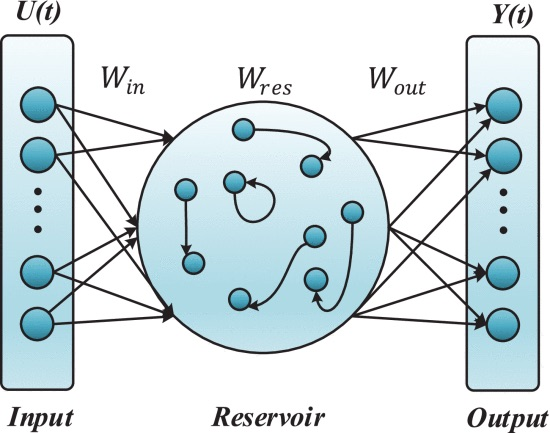
\includegraphics[scale=0.25]{figs/ESN_im.jpeg}
    \caption{\citep{zheng2020long}}
    
    \label{fig:enter-label}
\end{figure}

\textbf{Question for Dr.Teuscher: Should I discuss basic hyper-parameters like leakage rate, spectral radius, etc, or should I stop adding further content to the introduction?}






\section{Review of Each Framework}
\subsection{ReservoirPy}
ReservoirPy is a RC framework developed by \cite{Trouvain2020} with the support of INRIA with the purpose of providing an interface for both novices and experts to implement highly customizable ESN architectures. It is currently being maintained and was updated as recently as September 26th, 2023. The main back-end dependency of ReservoirPy is NumPy - a popular open source library of used for rapid numerical computation tailored for multidimesional arrays. 
\subsubsection{Important Features}
ReservoirPy has unique back-end features that have been specifically implemented to improve performance. These back-end features are:
\begin{itemize}
  \item Sparse matrix computation:  
  \item Fast spectral initialization:
  \item Parallel computation of states within reservoir:
\end{itemize}
These features, while important do not directly impact the user's implementation of RCs.

ReservoirPy has many features that are important for users to be familiar with for the purposes of implementing customizable RCs. These features are:
\begin{itemize}
  \item Custom/general offline or online training
  \item Ability to implement specific feedback connection such as the addition of input to readout feedback and specific feedback connections
  \item Support of deep architectures besides just reservoir to readout connections such multi-reservoir ESNs, multi-input-ESNs, etc.
  \item Support for unique implementations of reservoir and readout layers through the node class
  \item Support for hyperparameter optimization 
  \item In-built compatibility with specfic sklearn estimators
\end{itemize}

\subsubsection{Tutorials}
ReservoirPy has a comprehensive set of  tutorials, most of which are found within the ReservoirPy documentation. However, there are some additional tutorials available on the ReservoirPy Github page. The tutorials demonstrate the basic functionality of ReservoirPy. Demonstrations of each of the advanced features are included as part of the tutorials. Also, demonstrations of the use of the framework for novel tasks such as spoken vowel classification, 10 time-step generative forecasting.




ReservoirPy documentation can be accessed from the following link: \url{https://reservoirpy.readthedocs.io/en/latest/index.html}
The github link for ReservoirPy: 

\subsubsection{Installation}
Pip is the method of installation recommended for installing ReservoirPy. Pip should be used to download ReservoirPy into whichever environment is being used to run ReservoirPy based simulations.

ReservoirPy cannot be installed in a conda environment, must use venv or virtual environment.





\subsection{pyRCN}
 pyRCN is a lightweight RC framework developed by \cite{steiner2021pyrcn}. pyRCN is inspired by ReservoirPy; however, the scope of pyRCN is different. pyRCN intends to eventually provide the building blocks from which any RC architecture can be build such as ESNs, LSMs, Extreme Learning Machines (ELMs), and Deep RC networks. Currently pyRCN can be used to implement ESNs, ELMs, and deep architectures. It has been most recently maintained as of August 22, 2022. This framework's main dependencies are the scipy and numpy packages.
 
\subsubsection{Important Features}

pyRCN provides the following features for users to simulate RCs:
\begin{itemize}
    \item Support for hyperparameter optimization
    \item Support for deep architectures
    \item Single line implementation support for ESNClassifiers and ESNResgressors, and ELMClassifiers and ESNResgressors
    \item Fully compatible with scikit-learn interfaces
\end{itemize}

\subsubsection{Tutorials}
Of the frameworks, compared pyRCN provides the greatest number of tutorials with a total of 23 unique tutorials. These tutorials demonstrate features like hyperparameter optimization, simple ELM and ESN implementaion, and the use of sklearn estimators and hyperparameter optimization algorithms.

\subsubsection{Installation}
pyRCN can be installed using pip into a virtual environment. 


\subsection{RcTorch}
RcTorch is a Pytorch dependant RC simulation framework developed by \cite{joy2022rctorch}. This RC framework was created with the specific task of solving differential equations using RC with a specially implemented Bayesian Optimization algorithm used to tune hyperparameters. This framework was last updated on January 1st, 2023
 
\subsubsection{Important Features}
RcTorch has a minimal set of features:

\begin{itemize}
    \item In-built Bayesian Optimization of hyperparameters
    \item Support for ESN architectures built for the specific task of solving differential equations
\end{itemize}
\subsubsection{Tutorials}
RcTorch provides an extremely limited set of tutorials that show how the framework can be utilized to create RCs that solve differential equations such as the forced pendulum, Bernouli's equation, and a non-linear oscillator.

No time-series prediction or classification task is shown to be done with the RcTorch framework.
\subsubsection{Installation}
RcTorch is installed through the use of pip into a virtual environment


\subsection{pytorch-esn}
pytorch-esn is an RC simulation framework with PyTorch as its main dependency. This RC framework was developed by Stefano Nardo as a part of his masters thesis at the University of Pisa. This RC framework has been updated last on Febuary 17th, 2023

\subsubsection{Important Features}
Features for specific RC implementation are:
\begin{itemize}
    \item Support for deep architectures
    \item Readout layer compatible with pytorch optimizers
\end{itemize}
\subsubsection{Tutorials}
This RC framework provides only 2 tutorials. The first tutorial depicting how the framework can by use to simulate an RC to complete the Mackey-Glass 1 step timeseries prediction task. The second tutorials provides the code for simulating an RC to classify the values associated with digits from the MNIST dataset.
\subsubsection{Installation}
This RC framework cannot be installed with pip. Instead, the framework must be cloned from git and placed in the directory in which there are files that require access to this module.  

\subsection{ReservoirComputing.jl}
ReservoirComputing.jl was written in the Julia language with the SciML Julia machine learning package as its main dependency. ReservoirComputing.jl was developed by \cite{JMLR:v23:22-0611} and was introduced in the Journal of Machine Learning Research. The framework was last updated on October 28th, 2023
\subsubsection{Important Features}
ReservoirComputing.jl has a variety of features that allow specific implementations of ESNs:
\begin{itemize}
    \item Multiple training algorithms for RC readout layer
    \item Support for generative predictive models in addition to simple 1 step predictive models
    \item Support for modifying the internal state of the reservoir during training
    \item Support for different implementations of reservoirs
    \item Support for deep architectures
\end{itemize}
\subsubsection{Tutorials}
ReservoirComputing.jl has a set of tutorials demonstrating all of its features. Tutorials are provided for completing single step time-series predictions and multi-step time series predictions. No tutorial was created for classification tasks


\subsubsection{Installation}
Will have Hara write this section 

\section{Comparison Table of RC frameworks}
\begin{center}
\begin{tabular}{ | m{5em} | m{1cm}| m{1cm} | } 
  \hline
  cell1 dummy text dummy text dummy text& cell2 & cell3 \\ 
  \hline
  cell1 dummy text dummy text dummy text & cell5 & cell6 \\ 
  \hline
  cell7 & cell8 & cell9 \\ 
  \hline
\end{tabular}
\end{center}
\section{Testing Methodology}
\subsection{Training Tasks}
\subsection{Measurements of Performance}
\section{Results}
\section{Discussion}


\section{Conclusion}
\section{Acknowledgements}



\section{Bibliography styles}


There are various bibliography styles available. You can select the
style of your choice in the preamble of this document. These styles are
Elsevier styles based on standard styles like Harvard and Vancouver.
Please use Bib\TeX\ to generate your bibliography and include DOIs
whenever available.

Here are two sample references: 
\citep{Fortunato2010}
\cite{Fortunato2010,NewmanGirvan2004}
\cite{Fortunato2010,Vehlowetal2013}




  





\section{Bibliography}

Two bibliographic style files (\verb+*.bst+) are provided ---
{model1-num-names.bst} and {model2-names.bst} --- the first one can be
used for the numbered scheme. This can also be used for the numbered
with new options of {natbib.sty}. The second one is for the author year
scheme. When  you use model2-names.bst, the citation commands will be
like \verb+\citep+,  \verb+\citet+, \verb+\citealt+ etc. However when
you use model1-num-names.bst, you may use only \verb+\cite+ command.

\verb+thebibliography+ environment.  Each reference is a\linebreak
\verb+\bibitem+ and each \verb+\bibitem+ is identified by a label,
by which it can be cited in the text:

\noindent In connection with cross-referencing and
possible future hyperlinking it is not a good idea to collect
more that one literature item in one \verb+\bibitem+.  The
so-called Harvard or author-year style of referencing is enabled
by the \LaTeX{} package {natbib}. With this package the
literature can be cited as follows:

\begin{enumerate}[\textbullet]
\item Parenthetical: \verb+\citep{WB96}+ produces (Wettig \& Brown, 1996).
\item Textual: \verb+\citet{ESG96}+ produces Elson et al. (1996).
\item An affix and part of a reference:\break
\verb+\citep[e.g.][Ch. 2]{Gea97}+ produces (e.g. Governato et
al., 1997, Ch. 2).
\end{enumerate}

In the numbered scheme of citation, \verb+\cite{<label>}+ is used,
since \verb+\citep+ or \verb+\citet+ has no relevance in the numbered
scheme.  {natbib} package is loaded by {cas-dc} with
\verb+numbers+ as default option.  You can change this to author-year
or harvard scheme by adding option \verb+authoryear+ in the class
loading command.  If you want to use more options of the {natbib}
package, you can do so with the \verb+\biboptions+ command.  For
details of various options of the {natbib} package, please take a
look at the {natbib} documentation, which is part of any standard
\LaTeX{} installation.

\appendix
\section{My Appendix}
Appendix sections are coded under \verb+\appendix+.

\verb+\printcredits+ command is used after appendix sections to list 
author credit taxonomy contribution roles tagged using \verb+\credit+ 
in frontmatter.

\printcredits

%% Loading bibliography style file
%\bibliographystyle{model1-num-names}
\bibliographystyle{cas-model2-names}

% Loading bibliography database
\bibliography{RC_ref}




\bio{figs/pic1}
Author biography with author photo.
Author biography. Author biography. Author biography.
Author biography. Author biography. Author biography.
Author biography. Author biography. Author biography.
Author biography. Author biography. Author biography.
\endbio

\end{document}

